\documentclass[11pt,a4paper,reqno]{amsart}

\usepackage[utf8]{inputenc}
\usepackage[T1]{fontenc}
\usepackage{lmodern}
\usepackage{amsmath,amssymb,amsthm}
\usepackage{graphicx}
\usepackage[margin=28mm]{geometry}
\usepackage{xurl}
\usepackage[hidelinks]{hyperref}
\usepackage{orcidlink}
\usepackage{microtype}

\newtheorem{theorem}{Theorem}[section]
\newtheorem{proposition}[theorem]{Proposition}
\newtheorem{lemma}[theorem]{Lemma}
\newtheorem{corollary}[theorem]{Corollary}
\newtheorem{conjecture}[theorem]{Conjecture}
\theoremstyle{definition}
\newtheorem{question}[theorem]{Question}
\newtheorem{example}[theorem]{Example}
\theoremstyle{remark}
\newtheorem{remark}[theorem]{Remark}
\numberwithin{equation}{section}

\newcommand{\ggr}{\gamma_{\mathrm{gr}}}
\newcommand{\sprod}{\boxtimes}
\newcommand{\oct}{K_{2,2,2}}
\newcommand{\F}{\mathbb{F}}
\newcommand{\Z}{\mathbb{Z}}

\title[Strong-product ratios for the Grundy domination number]{Unbounded strong-product ratios for the Grundy domination number}

\author{Deep Bhattacharjee\,\orcidlink{0000-0003-0466-750X}}
\address{Formerly, Electro-Gravitational Space Propulsion Laboratory (EGSPL), Bhubaneswar, Odisha 751030, India}
\address{Formerly, University of Calcutta, Senate House, 87/1 College Street, Kolkata 700073, West Bengal, India}
\email{d.bhattacharjee@erl-forschung.de}
\email{itsdeep@live.com}
\email{egspl@proton.me}
\thanks{\sloppy Corresponding author: Deep Bhattacharjee. Email: \href{mailto:d.bhattacharjee@erl-forschung.de}{d.bhattacharjee@erl-forschung.de}, \href{mailto:itsdeep@live.com}{itsdeep@live.com}, \href{mailto:egspl@proton.me}{egspl@proton.me}; ORCID \href{https://orcid.org/0000-0003-0466-750X}{0000-0003-0466-750X}.}

\subjclass[2020]{05C69; 05C76}
\keywords{Grundy domination number; strong product; dominating sequence; incidence matrix}
\date{26 October 2026}

\begin{document}

\begin{abstract}
\itshape
A sequence of vertices of a graph is legal when every vertex in it dominates some vertex that none of the earlier ones dominated, and the Grundy domination number of the graph is the length of its longest legal sequence. In the strong product of two graphs, two vertices are adjacent when each coordinate is equal or adjacent in its factor. It has been known since 2016 that the Grundy domination number of a strong product is at least the product of the Grundy domination numbers of the two factors, and it was conjectured, by Bre\v{s}ar, Bujt\'as, Gologranc, Klav\v{z}ar, Ko\v{s}mrlj, Patk\'os, Tuza and Vizer, that equality always holds. We show that the conjecture is false, and false by an unbounded factor: for every number $C$ there are graphs whose strong product has Grundy domination number more than $C$ times the product of the two factors. The graphs are built on the five-element subsets of an $m$-element set, with adjacency decided by the size of the intersection; incidence matrices over the fields with two and three elements bound the two factors by $m$ and $\binom m2$, while the diagonal of the product is an independent set of size $\binom m5$. We also compute the Grundy domination number of the graph on $\{0,\dots,N-1\}$ in which $u$ and $v$ are adjacent when $|u-v|\equiv2\pmod3$: it is $\lfloor(N+1)/3\rfloor+3$ for every $N\ge6$. Its strong product with the octahedron has a legal sequence of length $N$, so the conjecture already fails for $N=19$, on a graph with $114$ vertices, and for every $N\ge21$. Every statement is proved by hand.
\end{abstract}

\maketitle



\medskip
\begin{quote}
\small\sloppy
\noindent\textbf{Note.} The counterexample of this paper was first made public on 14 October 2026, as release \texttt{v1.0.0} of the repository \url{https://github.com/creelie/grundy-strong-product}, archived on Zenodo as \href{https://doi.org/10.5281/zenodo.23378021}{10.5281/zenodo.23378021}. An earlier and incomplete version of the paper appeared on Hexagon on 23 October 2026 as the preprint \texttt{hexagon:2610.00494}, available at \url{https://hexagonmath.org/2610.00494}. That version gave one counterexample, the strong product of the octahedron with the graph $H_{21}$ on $21$ vertices, and relied on a computer certificate for the Grundy domination number of $H_{21}$. The revisions that followed are archived on Zenodo as \href{https://doi.org/10.5281/zenodo.23607502}{10.5281/zenodo.23607502} and \href{https://doi.org/10.5281/zenodo.23629621}{10.5281/zenodo.23629621}, in the repository \url{https://github.com/creelie/Paper_1}. This version is complete and self-contained: the Grundy domination number of $H_N$ is computed by hand for every $N\ge6$, the ratio is shown to be unbounded, the scope of each result is stated, no statement rests on a computer, and the only unrefereed source it depends on is the withdrawn proof claim that it mentions for the record. The source of this revision is in the repository named in the data availability statement at the end, archived on Zenodo as \href{https://doi.org/10.5281/zenodo.23659882}{10.5281/zenodo.23659882} (concept \href{https://doi.org/10.5281/zenodo.23607651}{10.5281/zenodo.23607651}), together with programs that recompute the small cases.
\end{quote}

\section{Introduction}\label{sec:intro}

Let $G$ be a finite simple graph and write $N[v]$ for the closed neighbourhood of a vertex $v$, the set consisting of $v$ and its neighbours. A sequence $(v_1,\dots,v_k)$ of vertices of $G$ is \emph{legal} if every $v_i$ dominates a vertex that none of its predecessors dominates, that is,
\[
  N[v_i]\setminus\bigcup_{j<i}N[v_j]\neq\emptyset\qquad(1\le i\le k);
\]
a vertex in this difference is a \emph{footprint} of $v_i$.\footnote{A vertex may have several footprints; any one of them witnesses that the step is legal. The vertices of a legal sequence are distinct, since a repeated vertex dominates nothing new.} The \emph{Grundy domination number} $\ggr(G)$ is the length of a longest legal sequence; a longest legal sequence always dominates $G$, since otherwise an undominated vertex could be appended. The parameter was introduced by Bre\v{s}ar, Gologranc, Milani\v{c}, Rall and Rizzi~\cite{BGMRR}, who connected it with the domination game.

In the strong product $G\sprod H$ two distinct vertices $(g,h)$ and $(g',h')$ are adjacent when $g'\in N_G[g]$ and $h'\in N_H[h]$; equivalently $N_{G\sprod H}[(g,h)]=N_G[g]\times N_H[h]$. Taking a Grundy dominating sequence of $G$ and one of $H$ and listing their pairs in lexicographic order gives a legal sequence of $G\sprod H$, so
\begin{equation}\label{eq:lower}
  \ggr(G\sprod H)\ \ge\ \ggr(G)\,\ggr(H)
\end{equation}
for all $G$ and $H$~\cite[Proposition~21]{BBG}.\footnote{If $d_i$ footprints $u_i$ in $G$ and $d'_j$ footprints $u'_j$ in $H$, then $(d_i,d'_j)$ footprints $(u_i,u'_j)$ in the lexicographic order of the pairs, because an earlier pair $(d_a,d'_b)$ has $a<i$, so $u_i\notin N[d_a]$, or $a=i$ and $b<j$, so $u'_j\notin N[d'_b]$.} In the same paper the authors conjectured that the bound is always attained.

\begin{conjecture}[{\cite[Conjecture~22]{BBG}}]\label{conj}
For all graphs $G$ and $H$, $\ggr(G\sprod H)=\ggr(G)\,\ggr(H)$.
\end{conjecture}

The conjecture holds when $G$ is a caterpillar~\cite{BBG} and, more generally, when $G$ is a forest, by the work of Bell, Driscoll, Krop and Wolff~\cite{BDKW}. A proof for all graphs was announced by Herrman and Smith~\cite{HS} and later withdrawn.\footnote{The second version of arXiv:2212.04565 (12 January 2023) carries the comment ``There is an error. Some cases were not considered in the proof of Theorem~1.''} We show that the conjecture is false and that no constant multiple of its proposed value is an upper bound.

\begin{theorem}\label{thm:unbounded}
For every $C>0$ there are nonempty finite graphs $G,H$ such that
\[
 \ggr(G\sprod H)>C\,\ggr(G)\ggr(H).
\]
\end{theorem}

Section~\ref{sec:unbounded} proves this with two graphs on the five-element subsets of $\{1,\dots,m\}$. Each factor is bounded through an incidence matrix over a finite field whose nonzero entries are exactly the closed neighbourhoods, and the diagonal of the product is an independent set. The ratio grows like $m^2$.

The smallest counterexamples we know come from a different construction, with the octahedron as first factor. For $N\ge1$ let $H_N$ be the graph on $\{0,1,\dots,N-1\}$ in which $u$ and $v$ are adjacent when $|u-v|\equiv2\pmod 3$, and let $\oct$ be the octahedron, the complete tripartite graph with three parts of size two. We compute the Grundy domination number of $H_N$ for every order.

\begin{theorem}\label{thm:family}
For every $N\ge6$,
\[
 \ggr(H_N)=\Big\lfloor\frac{N+1}{3}\Big\rfloor+3.
\]
Moreover $\ggr(\oct\sprod H_N)\ge N$ for every $N\ge1$. Thus Conjecture~\ref{conj} fails for $N=19$ and for every $N\ge21$.
\end{theorem}

The proof is in Sections~\ref{sec:graphs} to~\ref{sec:family}. After the first vertex of a legal sequence is chosen in a suitable circulant graph containing $H_N$, the undominated vertices form a half graph, and a count at the first selected edge, or an injection at the first selected vertex of the third residue class, gives the upper bound. Explicit sequences attain it. At $N=19$ the factors have Grundy domination numbers $2$ and $9$, while their product has a legal sequence of length $19$. This is a counterexample on $114$ vertices. By Proposition~25 of~\cite{BBG}, $\ggr(G\sprod H)\le|V(G)|\,\ggr(H)$, so with the octahedron as first factor the ratio is at most $3$; Theorem~\ref{thm:unbounded} must vary both factors.

The arguments are elementary: rank bounds for matrices with prescribed support, and counting in a half graph. Counts of this kind, attached to a finite structure or a group action, also appear in the author's earlier work~\cite{Bha22a,Bha22b,BB26}.

\section{Unbounded product ratios}\label{sec:unbounded}

To obtain unbounded ratios we vary both factors. The factor bounds come from incidence matrices over different fields, in the manner of the intersection-congruence arguments used by Alon~\cite[Section~3]{Alon} for the Shannon capacity; the application here needs the nonzero entries to be exactly the closed neighbourhoods, so that every legal sequence, and not only every independent set, is bounded. No result about the Shannon capacity is used.

\begin{lemma}\label{lem:rank}
Let $G$ be a finite graph and let $M$ be a matrix over a field $\F$, with rows and columns indexed by $V(G)$. Suppose that
\[
 M_{uv}\ne0\quad\Longleftrightarrow\quad v\in N_G[u].
\]
Then $\ggr(G)\le\operatorname{rank}_{\F}M$.
\end{lemma}

\begin{proof}
Let $(v_1,\dots,v_k)$ be legal and choose a footprint $w_i$ for each $v_i$. The footprints are distinct, since $w_j$ is not dominated by $v_1,\dots,v_{j-1}$ while $w_i\in N[v_i]$ for $i<j$. If $i<j$, then $w_j\notin N_G[v_i]$, so $M_{v_iw_j}=0$, and each $M_{v_iw_i}$ is nonzero. The submatrix with rows $v_1,\dots,v_k$ and columns $w_1,\dots,w_k$, in this order, is lower triangular with nonzero diagonal, so its rank is $k$, and $k\le\operatorname{rank}M$.
\end{proof}

The condition on $M$ cannot be weakened to vanishing on non-edges: the footprint $w_i$ need not equal $v_i$, so the entries $M_{uv}$ with $v$ a neighbour of $u$ must be nonzero as well.\footnote{For an independent set the diagonal alone would do; this is the difference between bounding the independence number, as in the Shannon capacity arguments, and bounding the Grundy domination number.}

\begin{theorem}\label{thm:two-fields}
For $m\ge5$, let $A_m$ and $B_m$ have vertex set $\binom{[m]}5$, the five-element subsets of $[m]=\{1,\dots,m\}$. Distinct sets $S,T$ are adjacent in $A_m$ when $|S\cap T|$ is odd, and in $B_m$ when $|S\cap T|\equiv2\pmod3$. Then
\[
 \ggr(A_m)\le m,\qquad \ggr(B_m)\le\binom m2,\qquad
 \ggr(A_m\sprod B_m)\ge\binom m5.
\]
In particular,
\begin{equation}\label{eq:unbounded-ratio}
 \frac{\ggr(A_m\sprod B_m)}{\ggr(A_m)\ggr(B_m)}
 \ge\frac{(m-2)(m-3)(m-4)}{60m},
\end{equation}
so the ratios are unbounded.
\end{theorem}

\begin{proof}
Let $U$ be the incidence matrix between five-element subsets of $[m]$ and elements of $[m]$, with $U_{Sx}=1$ when $x\in S$. Over $\F_2$,
\[
 (UU^{\mathsf T})_{ST}=|S\cap T|\pmod2.
\]
Since $|S|=5$ is odd, the diagonal entries are nonzero, and an off-diagonal entry is nonzero exactly when $|S\cap T|$ is odd, that is, when $S$ and $T$ are adjacent in $A_m$. So the nonzero entries of $UU^{\mathsf T}$ are exactly the closed neighbourhoods of $A_m$. Its rank is at most the number $m$ of columns of $U$, and Lemma~\ref{lem:rank} gives the first bound.

Let $V$ be the incidence matrix between five-element subsets and two-element subsets of $[m]$, with $V_{SP}=1$ when $P\subseteq S$. Over $\F_3$,
\[
 (VV^{\mathsf T})_{ST}=\binom{|S\cap T|}{2}\pmod3,
\]
the number of two-element subsets of $S\cap T$. For intersection sizes $t=0,1,2,3,4,5$ the values $\binom t2=0,0,1,3,6,10$ reduce to $0,0,1,0,0,1$ modulo $3$. So the entry is nonzero exactly when $S=T$ or $|S\cap T|=2$, which are precisely the closed neighbourhoods of $B_m$. The rank is at most $\binom m2$, proving the second bound.

The product vertices
\[
 \mathcal D_m=\{(S,S):S\in\tbinom{[m]}5\}
\]
form an independent set of $A_m\sprod B_m$: for $S\ne T$, adjacency of $(S,S)$ and $(T,T)$ would need $S$ and $T$ adjacent in both factors, which would require $|S\cap T|$ to be $1$ or $3$ and also $2$. Listing the vertices of $\mathcal D_m$ in any order gives a legal sequence, each vertex footprinting itself, because no earlier vertex of the list dominates it. This proves the lower bound $\binom m5$ for the product.

The three bounds give~\eqref{eq:unbounded-ratio}, since
\begin{align*}
&\binom m5\Big/\Bigl(m\binom m2\Bigr)\\
 &=\frac{m(m-1)(m-2)(m-3)(m-4)}{120}\cdot\frac{2}{m^2(m-1)}\\
 &=\frac{(m-2)(m-3)(m-4)}{60m},
\end{align*}
and the right side tends to infinity with $m$.
\end{proof}

\begin{proof}[Proof of Theorem~\ref{thm:unbounded}]
Take $G=A_m$ and $H=B_m$ with $m$ so large that $(m-2)(m-3)(m-4)>60Cm$.
\end{proof}

For example, $m=13$ gives $\ggr(A_{13}\sprod B_{13})\ge1287$, whereas $\ggr(A_{13})\ggr(B_{13})\le13\cdot78=1014$. The two factor bounds use different fields; no matrix product over a common field is involved, and nothing is claimed about the exact values of $\ggr(A_m)$ and $\ggr(B_m)$.

\section{The octahedron and the graphs \texorpdfstring{$H_N$}{HN}}\label{sec:graphs}

We write the vertices of the octahedron as $g_0,g_1,g_2,x_0,x_1,x_2$, where $x_t$ is the antipode of $g_t$; the three antipodal pairs are the only non-adjacent pairs (Figure~\ref{fig:oct}). Thus $N[v]$ is everything except the antipode of $v$.

\begin{figure}[ht]
\centering
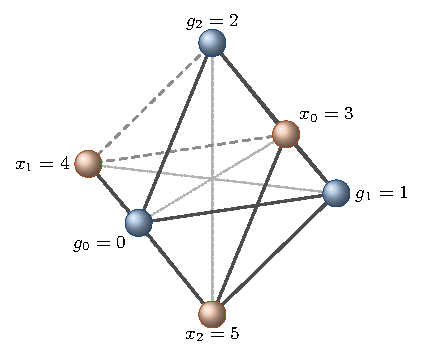
\includegraphics[width=0.42\textwidth]{figures/octahedron.pdf}
\caption{The octahedron $\oct$. Each vertex is adjacent to all others except its antipode; the dotted segments join the antipodal pairs $\{g_t,x_t\}$.}\label{fig:oct}
\end{figure}

\begin{lemma}\label{lem:oct}
$\ggr(\oct)=2$.
\end{lemma}

\begin{proof}
The sequence $(g_0,x_0)$ is legal: $x_0$ footprints itself. Conversely, let $(u,v)$ be legal. If $v$ is the antipode of $u$, then $N[u]\cup N[v]$ is the whole vertex set; otherwise $N[u]$ misses only the antipode of $u$, which lies in $N[v]$. Either way nothing is left for a third vertex to footprint.
\end{proof}

In $H_N$ we write $a_i=3i$, $b_i=3i+1$ and $c_i=3i+2$. Two vertices of the same residue class modulo $3$ are never adjacent, and for vertices of different classes
\begin{equation}\label{eq:adj}
  a_i\sim c_j\iff j\ge i,\qquad b_i\sim a_j\iff j>i,\qquad c_i\sim b_j\iff j>i,
\end{equation}
because $c_j-a_i=3(j-i)+2$, $a_j-b_i=3(j-i)-1$ and $b_j-c_i=3(j-i)-1$, and a difference $3k-1$ with $k\le0$ has absolute value $3|k|+1\equiv1\pmod3$.

\section{A long legal sequence in the product}\label{sec:product}

The construction uses one property of $H_N$: with the colouring $v\mapsto v\bmod 3$, every edge $uv$ with $u<v$ satisfies $u\equiv v+1\pmod 3$, since $v-u\equiv2$. We state it for any graph with this property.

\begin{proposition}\label{prop:product}
Let $H$ be a graph with vertices $v_0,\dots,v_{N-1}$ and a map $t\colon V(H)\to\Z_3$ such that $t(v_i)\equiv t(v_j)+1\pmod3$ for every edge $v_iv_j$ with $i<j$. Then the sequence
\[
  s_j=\big(g_{t(v_j)},\,v_j\big),\qquad j=0,1,\dots,N-1,
\]
is legal in $\oct\sprod H$, and $\ggr(\oct\sprod H)\ge N$. In particular $\ggr(\oct\sprod H_N)\ge N$ for every $N\ge1$, with $t(v)=v\bmod3$.
\end{proposition}

\begin{proof}
We show that $s_j$ footprints $f_j=(x_{t(v_j)+1},v_j)$, the indices of $g$ and $x$ being taken modulo $3$. First, $f_j\in N[s_j]$: the vertex $x_{t(v_j)+1}$ is not the antipode $x_{t(v_j)}$ of $g_{t(v_j)}$, so it lies in $N[g_{t(v_j)}]$, and $v_j\in N[v_j]$. Now let $i<j$. If $f_j\in N[s_i]$, then $x_{t(v_j)+1}\in N[g_{t(v_i)}]$, which means $t(v_i)\ne t(v_j)+1$, and $v_j\in N[v_i]$, which for $i\ne j$ means that $v_iv_j$ is an edge, hence $t(v_i)=t(v_j)+1$. The two conclusions contradict each other, so $f_j\notin N[s_i]$.
\end{proof}

Figure~\ref{fig:product} shows the sequence for $H_{21}$. Every column of the product contains exactly one vertex of the sequence, while a sequence of the form used for~\eqref{eq:lower} would use only $\ggr(H_{21})=10$ columns. The rotation of the three colours along the sequence is what lets each new vertex reach a footprint in a layer $x_t$ that none of the earlier vertices covers in that column.

\begin{figure}[ht]
\centering
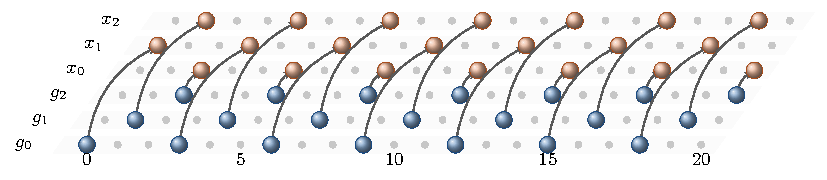
\includegraphics[width=\textwidth]{figures/product.pdf}
\caption{$\oct\sprod H_{21}$ as six stacked copies of $H_{21}$, one for each vertex of the octahedron. The $21$ blue vertices $(g_{j\bmod3},j)$ form a legal sequence; the arrow from each of them ends at its footprint $(x_{(j+1)\bmod 3},j)$.}\label{fig:product}
\end{figure}

\section{The Grundy domination number of \texorpdfstring{$H_N$}{HN}}\label{sec:family}

We prove the formula of Theorem~\ref{thm:family} for every $N\ge6$. A legal sequence in an induced subgraph remains legal in the larger graph, with the same footprints, since closed neighbourhoods in the subgraph are the intersections of those in the larger graph with the subgraph. We use this observation for both bounds.

\begin{lemma}\label{lem:upper-all}
For every integer $q\ge1$, $\ggr(H_{3q+1})\le q+3$.
\end{lemma}

\begin{proof}
Put $n=3q+1$. For $1\le d<n$, the conditions $d\equiv2\pmod3$ and $n-d\equiv2\pmod3$ are equivalent, because $n\equiv1$. So $u$ and $v$ are adjacent in $H_n$ exactly when $(u-v)\bmod n$ lies in the set of residues congruent to $2$ modulo $3$, and translation modulo $n$ preserves adjacency.\footnote{For $u>v$ the difference $u-v=d$ and the residue $(v-u)\bmod n=n-d$ are both or neither congruent to $2$, so the adjacency condition $|u-v|\equiv2$ is the same as the circulant condition.} A legal sequence stays legal under a graph automorphism, so we may translate a nonempty legal sequence so that its first vertex is $0$.

The vertex $0$ dominates itself and the vertices $C_k=3k+2$, $0\le k<q$. The undominated vertices are
\[
 X_i=3(i+1),\qquad Y_j=3j+1\qquad(0\le i,j<q).
\]
There are no edges within either class, and
\begin{equation}\label{eq:half}
 X_i\sim Y_j\quad\Longleftrightarrow\quad i\ge j,
\end{equation}
because $X_i-Y_j=3(i-j)+2$ when $i\ge j$, and $Y_j-X_i=3(j-i-1)+1$ when $j>i$. Thus the undominated vertices induce a half graph with the perfect matching $X_iY_i$ (Figure~\ref{fig:half}).

\begin{figure}[tb]
\centering
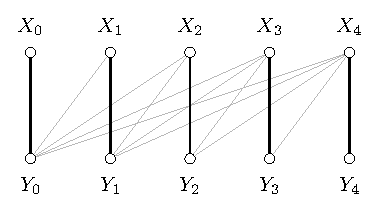
\includegraphics[width=0.85\textwidth]{figures/half-graph.pdf}
\caption{The undominated graph after selecting $0$ in $H_{3q+1}$, drawn for $q=5$. The matching edges $X_iY_i$ are emphasised. Before the first selected edge, every selected $X$-index is smaller than every selected $Y$-index.}\label{fig:half}
\end{figure}

Follow the sequence from its second vertex on until either a vertex $C_k$ is selected or the selected $X$- and $Y$-vertices contain an edge for the first time. Before either event, let $I$ and $J$ be the sets of selected indices on the two sides, and put $r=|I|$, $s=|J|$. By~\eqref{eq:half}, the absence of edges means
\begin{equation}\label{eq:independent}
 i<j\qquad(i\in I,\ j\in J).
\end{equation}
We treat the three possibilities in turn.

\emph{A new $X_i$ creates an edge.} Then $J\ne\emptyset$ and $b=\min J\le i$. All earlier $X$-indices are less than $b$ by~\eqref{eq:independent}, so $i$ is the largest selected $X$-index. After this step, an $X$-vertex is dominated if it was selected or if it is adjacent to a selected $Y_j$, that is, if its index is at least $b$; so the undominated $X$-indices are $\{0,\dots,b-1\}\setminus I$. A $Y$-vertex is dominated if it was selected or is adjacent to a selected $X$-vertex, and the selected $X$-vertex with the largest index is $X_i$; so the undominated $Y$-indices are those greater than $i$ that are not in $J$. Writing $s_0=|J\cap\{b,\dots,i\}|$ for the number of selected $Y$-indices at most $i$, the number of undominated vertices is
\[
 (b-r)+(q-1-i)-(s-s_0).
\]
The number of vertices selected after $0$, which is $r+s+1$, plus the number still undominated, is
\[
r+s+1+b-r+q-1-i-s+s_0=q+b-i+s_0\le q+1,
\]
because $s_0\le i-b+1$. Each later legal step dominates at least one vertex that was undominated, so the number of later steps is at most the number of undominated vertices. The full sequence, including its first vertex $0$, has length at most $1+(q+1)=q+2$.

\emph{A new $Y_j$ creates an edge.} The map $X_i\mapsto Y_{q-1-i}$, $Y_j\mapsto X_{q-1-j}$ exchanges the two sides and preserves~\eqref{eq:half}, since $q-1-j\ge q-1-i$ exactly when $i\ge j$. It carries this case to the previous one, so again the sequence has length at most $q+2$.

\emph{A vertex $C_k$ is selected first.} By~\eqref{eq:adj}, the neighbours of $C_k=c_k$ among the $X$- and $Y$-vertices are the $X_i=a_{i+1}$ with $i<k$ and the $Y_j=b_j$ with $j>k$. After this step every vertex still undominated belongs to
\[
W_k=\{X_i:k\le i<q\}\cup\{Y_j:0\le j\le k\},\qquad |W_k|=q+1.
\]
At least $r+s$ vertices of $W_k$ were dominated already before $C_k$ was selected. To see this, map each earlier selection by
\[
 X_i\longmapsto\begin{cases}X_i,&i\ge k,\\Y_i,&i<k,\end{cases}
 \qquad
 Y_j\longmapsto\begin{cases}Y_j,&j\le k,\\X_j,&j>k.\end{cases}
\]
Each image lies in $W_k$ and is either the selected vertex itself or its partner in the matching, which the selected vertex dominates by~\eqref{eq:half}. Images of distinct selections on the same side are distinct. An image shared by a selection $X_i$ and a selection $Y_j$ would force $i=j$, with $i\in I$ and $j\in J$, contrary to~\eqref{eq:independent}. So the map is injective, at most $q+1-r-s$ vertices remain undominated after $C_k$, and the sequence has length at most
\[
 1+(r+s)+1+(q+1-r-s)=q+3.
\]

\emph{Neither event occurs.} Then the vertices selected after $0$ form an independent set of the half graph, which has the perfect matching $X_iY_i$, so there are at most $q$ of them and the sequence has length at most $q+1$.

In every case the length is at most $q+3$.
\end{proof}

\begin{lemma}\label{lem:lower-all}
If $N\ge6$ and $q=\lfloor(N+1)/3\rfloor$, then $\ggr(H_N)\ge q+3$.
\end{lemma}

\begin{proof}
For $q=2$, the sequence $(1,3,5,0,2)$ in $H_6$ has the successive footprints $1,5,0,2,4$ and remains legal in $H_7$. For $q=3$, the sequence $(0,7,2,4,5,1)$ in $H_8$ has the successive footprints $0,7,4,6,3,1$ and remains legal in $H_9$ and $H_{10}$.\footnote{Each footprint can be checked from~\eqref{eq:adj}. In $H_6$, for instance, $1=b_0$ dominates $b_0$ and $a_1=3$; then $3=a_1$ dominates $a_1$, $c_1=5$ and $b_0$, so $5$ is new; $5=c_1$ dominates nothing new except itself, already dominated, so one checks instead that $c_1\sim b_j$ needs $j>1$, which does not exist, and $c_1\sim a_i$ needs $i\le1$, both already dominated; hence the third footprint is $0=a_0$, which $c_1$ dominates because $a_0\sim c_1$. The listed footprints are $1,5,0,2,4$ in this order: the first vertex $1$ footprints itself, $3$ footprints $5$, $5$ footprints $0$, $0$ footprints $2$, and $2$ footprints $4$.}

For $q\ge4$ it suffices to work in $H_{3q-1}$, which is an induced subgraph of $H_N$ because $3q-1\le N$. Its vertices are $a_i,b_i$ for $0\le i\le q-1$ and $c_i$ for $0\le i\le q-2$. Take the sequence
\begin{equation}\label{eq:lower-sequence}
 a_0,a_1,\dots,a_{q-3},\ b_{q-1},\ c_{q-3},\ c_0,\ a_{q-2},\ b_0 .
\end{equation}
The first $q-2$ vertices footprint themselves, since vertices of one class are never adjacent. The last five have the successive footprints
\[
 b_{q-1},\quad b_{q-2},\quad b_{q-3},\quad a_{q-2},\quad a_{q-1},
\]
by~\eqref{eq:adj}: $b_{q-1}$ is adjacent to no $a_i$ with $i\le q-3$, so it is undominated and footprints itself; $b_{q-2}$ is adjacent to $c_{q-3}$ and not to any earlier vertex of the sequence; $b_{q-3}$ is adjacent to $c_0$, because $q-3>0$, and not to $a_0,\dots,a_{q-3}$, $b_{q-1}$ or $c_{q-3}$; neither $a_{q-2}$ nor $a_{q-1}$ is adjacent to $b_{q-1}$, $c_{q-3}$ or $c_0$, so $a_{q-2}$ footprints itself and $b_0$ footprints $a_{q-1}$. The sequence has length $(q-2)+5=q+3$.
\end{proof}

\begin{proof}[Proof of Theorem~\ref{thm:family}]
Put $q=\lfloor(N+1)/3\rfloor$. Then $3q\le N+1$, so $N\le3q+1$ and $H_N$ is an induced subgraph of $H_{3q+1}$; Lemma~\ref{lem:upper-all} gives $\ggr(H_N)\le q+3$, and Lemma~\ref{lem:lower-all} gives equality. The product bound is Proposition~\ref{prop:product}.

At $N=19$ the formula gives $\ggr(H_{19})=9$, and $19>2\cdot9$. For $N\ge21$ write $N=3q-1$, $3q$ or $3q+1$; the differences $N-2(q+3)$ are $q-7$, $q-6$ and $q-5$, and each is positive in its range ($q\ge8$, $q\ge7$ and $q\ge7$ respectively). Hence $N>2\ggr(H_N)=\ggr(\oct)\ggr(H_N)$ for $N=19$ and every $N\ge21$, while $\ggr(\oct\sprod H_N)\ge N$.
\end{proof}

\begin{example}\label{ex:small}
For $N=19$ the sequence~\eqref{eq:lower-sequence} with $q=6$, in $H_{17}\subseteq H_{19}$, is $(0,3,6,9,16,\allowbreak11,2,12,1)$, of length $9=\ggr(H_{19})$, and $\oct\sprod H_{19}$ has $114$ vertices and a legal sequence of length $19$. For $N=21$, with $q=7$, the sequence is $(0,3,6,9,12,\allowbreak19,14,2,15,1)$, of length $10=\ggr(H_{21})$; this is the counterexample on $126$ vertices with which the paper began. For $N=20$ the formula gives $\ggr(H_{20})=10$ and $20=2\cdot10$, so Theorem~\ref{thm:family} says nothing about $N=20$.
\end{example}

\begin{remark}\label{rem:scope}
Everything above is proved in full. Theorem~\ref{thm:unbounded} rests on Lemma~\ref{lem:rank} and the two incidence matrices; Theorem~\ref{thm:family} on the half-graph count of Lemma~\ref{lem:upper-all}, the explicit sequences of Lemma~\ref{lem:lower-all} and Proposition~\ref{prop:product}. The only results quoted from elsewhere are the inequality~\eqref{eq:lower} and the bound $\ggr(G\sprod H)\le|V(G)|\ggr(H)$, both from~\cite{BBG} with proofs of a few lines, and neither is needed for the counterexamples themselves. Nothing is claimed about the exact values of $\ggr(A_m)$, $\ggr(B_m)$ or $\ggr(A_m\sprod B_m)$ beyond the three bounds, nor about the smallest possible counterexample.
\end{remark}

\section{A question}

\begin{question}
Which graphs $G$ satisfy Conjecture~\ref{conj} for every $H$? All forests do~\cite{BDKW}, whereas the octahedron does not.
\end{question}

\section*{Declarations}

\noindent\textbf{Funding.} None.

\smallskip
\noindent\textbf{Conflict of interest.} None.

\smallskip
\noindent\textbf{Data availability.} \url{https://github.com/creelie/Paper_1} (release \texttt{v2.0.0}, archived on Zenodo as \href{https://doi.org/10.5281/zenodo.23659882}{10.5281/zenodo.23659882}) holds the source of this paper and programs that recompute $\ggr(H_N)$ for small $N$ and check the sequences of Section~\ref{sec:family}; the paper does not depend on them.

\begingroup\sloppy\emergencystretch=3em\hbadness=5000
\begin{thebibliography}{99}

\bibitem{Alon}
N.~Alon, The Shannon capacity of a union, Combinatorica 18 (1998), no.~3, 301--310. \href{https://doi.org/10.1007/PL00009824}{doi:10.1007/PL00009824}.

\bibitem{BDKW}
K.~Bell, K.~Driscoll, E.~Krop and K.~Wolff, Grundy domination of forests and the strong product conjecture, Electron. J. Combin. 28 (2021), no.~2, Paper P2.12. \href{https://doi.org/10.37236/9507}{doi:10.37236/9507}.

\bibitem{Bha22a}
D.~Bhattacharjee, Establishing equivariant class $[O]$ for hyperbolic groups, Asian Res. J. Math. 18 (2022), no. 11, 362--369. \href{https://doi.org/10.9734/arjom/2022/v18i11615}{doi:10.9734/arjom/2022/v18i11615}.

\bibitem{Bha22b}
D.~Bhattacharjee, Non-commutativity over canonical suspension $\eta$ for genus $g\ge1$ in hypercomplex structures for potential $\rho\phi$, Asian Res. J. Math. 18 (2022), no. 11, 332--341. \href{https://doi.org/10.9734/arjom/2022/v18i11607}{doi:10.9734/arjom/2022/v18i11607}.

\bibitem{BB26}
D.~Bhattacharjee, U.~Bhattacharya, Iterated nerve complexes for $k$-fold sensor coverage, Preprints.org (2026). \href{https://doi.org/10.20944/preprints202606.1351.v2}{doi:10.20944/preprints202606.1351.v2}.

\bibitem{BBG}
B.~Bre\v{s}ar, Cs.~Bujt\'as, T.~Gologranc, S.~Klav\v{z}ar, G.~Ko\v{s}mrlj, B.~Patk\'os, Zs.~Tuza and M.~Vizer, Dominating sequences in grid-like and toroidal graphs, Electron. J. Combin. 23 (2016), no.~4, Paper P4.34. \href{https://doi.org/10.37236/6269}{doi:10.37236/6269}.

\bibitem{BGMRR}
B.~Bre\v{s}ar, T.~Gologranc, M.~Milani\v{c}, D.~F.~Rall and R.~Rizzi, Dominating sequences in graphs, Discrete Math. 336 (2014), 22--36. \href{https://doi.org/10.1016/j.disc.2014.07.016}{doi:10.1016/j.disc.2014.07.016}.

\bibitem{HS}
R.~Herrman and S.~G.~Z.~Smith, A proof of the Grundy domination strong product conjecture, \href{https://arxiv.org/abs/2212.04565v2}{arXiv:2212.04565} (2022), withdrawn in version 2 (12 January 2023).

\end{thebibliography}
\endgroup

\end{document}
